%overview
The ``software'' encompasses all programs that run on the scale units, the master unit, and the user interface client-side code. Despite the vast differences between these targets, the software had to be designed for maximum re-use. A number of feasibility studies were completed before the final approach was selected.

\subsection{Master Unit Considerations}
The master unit would run a full Linux operating systems, therefore more high-level languages and libraries could in theory be used.

Since the user interface was a web application, the master unit had to run a simple web-server that could serve the interface (HTML, Javascript, CSS files) as well as answer requests for dynamically generated information gathered from the scale units. As an initial prototype, the Python language with a webserver module \cite{bottle-py} was used. An open-source project \cite{webiopi} was discovered that would allow control of the GPIO pins and could potentially be adapted for this purpose. However, the serial port communication, and handling of single bytes for communicating with the radio transmitters were found to be insufficiently reliable and scalable.

Instead, it was decided to program the entire system in C, as this would allow for some portions of the code to be re-used on the scale units. This decision was affected by the fact that not much time was left to complete the project, and the web-server and client-side UI were deemed as optional features that could eventually be added in on top of this.

\subsection{Layered Approach}
A layered approach to the software architecture was taken. The system is modelled in three main layers, roughly following the OSI network systems model \cite{osi-model}. Each layer would define a well-known interface, and only the layer above would need to access this. Each layer can have several implementations to account for the fact that the embedded scale unit system would be very different from the Linux system on the master unit.

\begin{itemize}
	\item \textbf{Transport Layer:} The lowest layer maps primitive read and write methods to the underlying serial devices and provides buffering for incoming data.
	\item \textbf{Packet Layer:} This implements a packet protocol and provides methods for parsing incoming data, as well as packaging outgoing data.
	\item \textbf{Application Layer:} The highest layer implements the individual application functionality and defines responses to incoming packets, as well as interacting with other system components, such as the user interface or the analogue-to-digital converter.
\end{itemize}

\subsection{Packet Protocol}
The ZigBee protocol defines a wrapper packet protocol that is used for sending command and data frames across the serial link in the API mode \cite[page 35]{zigbee-datasheet}. This is then translated into another packet format used for over-the-air transmission.

ZigBee nodes can operate in two seperate modes. Firstly, transparent mode is the most basic communication, where only very basic pacektization is provided. However, this is very simple to get running for a basic point-to-point network. Unfortunately, once multiple nodes attempt to transmit at once, the packets become interleaved, rendering this mode not very useful for the envisioned network architecture. Still, it proved useful for initial debugging and manually sending data by connecting the device directly to a serial terminal.

Originally, a simple packet system was devised to run on top of the transparent mode. This was later found to be too unreliable and inefficient due to the aforementioned interleaving of data. Since this design was very similar to the ZigBee API protocol, few changes were required to send the payload data wrapped in packages conforming to this.

The payload consists of an \emph{Op-Code} to signify the current operation (ping, pong, measure request, measure response), a \emph{device identifier} that is set at compile-time, and the actual data in the case of a measure response. This data is encoded as, in this case four, hexadecimal ASCII characters rather than directly representing it as bytes. This decision was made to avoid having to escape control characters such as \texttt{7E} which defines the beginning of a packet in the ZigBee API. In the original design a length byte for the data was included, but this was abandoned since the wrapping API packet already contains a length field.

\subsection{User Interface}
The user interface to the system has been defined during the requirements gathering process to be a very simple web application that should support taking readings of the current system state by intitiating measurements, as well as providing simple calibration of the scales. Therefore a mock-up was drawn up, and based on this a static HTML/CSS prototype was generated (See figure \ref{fig-ui-screenshot}). This was then made interactive by attaching javascript actions to the buttons.

The client side application (the aforementioned javascript, running in a web-browser) would make asynchronous requests to special URLs on the server that are mapped to methods initiating data transfers between the master and scale units, or returning data previously stored on the server.

\begin{itemize}
	\item \texttt{/api/data} returns a JSON \cite{json-spec} object containing the data stored on the server for all sensors.
	\item \texttt{/api/calibrate} initiates a measurement on all scale units and sets the values received to be the zero-points for that particular sensor.
	\item \texttt{/api/measure} initiates a measurement and stores the results in a server-side structure to be later retreived by a \texttt{data} request.
\end{itemize}

It was decided that for the prototype, the master unit program was to be integrated with a previously (for Networked Systems 3 coursework \cite{ns3-webserver}) produced web server implementation, which should require minimal adjustments to support the added API functionality.

\subsection{Transport Layer}
The transport layer provides an interface to the serial link used to communicate with the ZigBee nodes.

\subsubsection{Exposed Transport API}
The interface used by higher layers is exposed through \texttt{zb\_transport.h}. It is modelled as a subset of the most common network operations, only implementing those required by the system -- that is, reading data as individual characters for passing them to the packet layer parser, and writing data as blocks of multiple bytes, for sending complete packets.

First of all, the system must be initialised using \texttt{zb\_transport\_init()}. Then data can be received character by character, in the order received, through the blocking \texttt{zb\_getc()} call. Finally, data can be sent to the device by providing an array of bytes and its size to \texttt{zb\_send()}. \texttt{zb\_transport\_stop()} has been added to perform clean-up operations such as closing file handles on implementations that require it.

\subsubsection{Linux Implementation}
Since the Raspberry Pi runs a complete Linux distribution (in this case, a stripped-down version of Raspbian, \cite{raspbian}, is used), the microprocessor's UART component is exposed as a serial port to the system, named \texttt{/dev/ttyAMA0}. This port can be accessed using standard file operation system calls such as \texttt{read} and \texttt{write} after having been initialised by opening the file and setting a number of standard serial options \cite{posix-serial-programming}.

A separate thread (implemented using pthreads) is running in the background, continuously monitoring the serial port by blocking on \texttt{read()}. Any characters are received on the port, these get stored in a thread safe bounded buffer structure from which they are retrieved by a higher layer implementation. Thread safety is ensured using pthread condition variables and locks.

\subsubsection{Bare Metal Implementation}
On the microcontroller, no threading capabilities besides raw interrupts are available, and the serial link is implemented as a peripheral component of the microcontroller. ST provides driver libraries for configuring and accessing such peripherals which have been used extensively for this implementation.

The USART peripheral provides a small hardware buffer that is currently used as the only buffer in this implementation due to the low frequency of packets and relatively short non-IO bursts in the software. Therefore, the \texttt{zb\_getc} implementation is currently busy-waiting for the memory-mapped USART status register to clear its \emph{RXNE} (Receive buffer non-empty) flag. This is a similiar structure to waiting for a condition variable in a pthread program. %TODO check if we can actually wait for interrupts here to put the processor to sleep, saving power and getting rid of bad busy waiting.

This is a polling method and using busy waiting, which is inherently using more power and is less flexible than waiting for interrupts. However, for prototyping and debugging, this made the testing and implementation much easier. It is expected that this can be re-developed using interrupts and additional software buffering. 

\subsection{Packet Layer}
The packet layer provides an abstraction for sending and receiving custom data in a fixed format (made up of an op-code, a sender identifier, and an arbitrary number of `data' bytes) over the transport layer. Its implementation is identical for all units, the only changes required are in the application layer's initialisation calls.

The first implementation, which was used for testing the transport layer due its simplicity, was based on a custom packet format that had nothing more than the aforementioned data content, a delimeter, and a checksum. The ZigBee units were pre-configured with destination addresses and options, and used in transparent mode.

Due to the issues explained in \ref{software-impl}, transparent mode had to be dropped and a second packet layer implementation tailored to the ZigBee API mode was developed using the same API calls. This is described in the following sections.

\subsubsection{Packet API}
The public API for the packet layer is defined in \texttt{zb\_packets.h}. 

Initialisation and settings are provided through the \texttt{zb\_packets\_init}, \texttt{zb\_set\_broadcast\_mode}, and \texttt{zb\_set\_device\_id} methods. In the current implementation, broadcast mode is the only way to set the target address: The master unit sends broadcast packages that are received by all scale units, and the scale units send unicast packages targeted only at the master unit. This state is held in a global variable, and it would be trivial to add functionality to support arbitrary target addresses, though this would require for the application layer to know about network or device addresses of the destination.

%TODO missing abstraction: Stop/close/destroy call should be to packets layer and handed down to transport.

\subsubsection{ZigBee Packet Structure and Parsing Methodology}
The ZigBee API defines data frames transmitted across the serial link between the host and ZigBee device. These packets are parsed and, if the packet is a transmission request, wrapped in a different 802.15.4 packet for transmission over the air, and re-packaged in a serial data frame on the other end.

Re-Transmission if checksums fail or no ACKs are received for these over-the-air packets is handled at the ZigBee layer that is equivalent to the Network layer in the OSI model, and in this implementation is completely independent from even the application transport layer. This was taken as a given as part of the decision to use the ZigBee devices and protocol, therefore the following discussion does not take this lower layer into account.

%TODO check with stuff I've already said above - get picture from data sheet/re-make in inkscape with our data.

Parsing of the incoming character stream is achieved through the \texttt{zb\_parse} method which must be called on every character received. It returns a status code to indicate when a complete packet has been received. At this point, globally available variables are filled with the relevant information (op code, device id, data, length) from the packet.

This method is implemented as a finite state machine with the state maintained in static local variables. This implementation is inspired by the Yacc parser/lexer architecture. In retrospect, these packages could well have been used for the implementation. Due to time constraints in the development phase, and initially starting off with a considerably smaller parser for the simpler packet structure, this was not fully considered before most of the implementation was completed. 

\subsection{Application Layer}
\begin{figure}
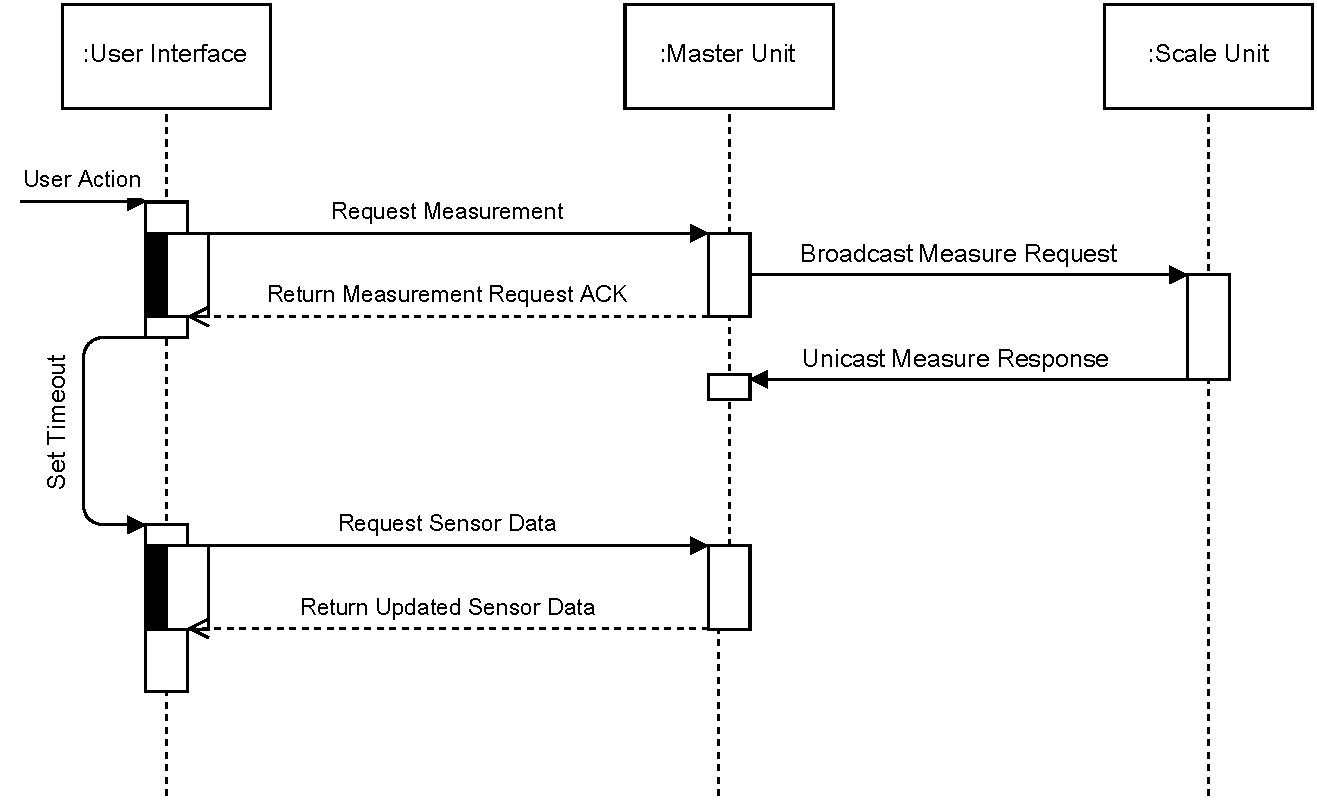
\includegraphics[width=\textwidth]{images/communications-diagram.pdf}
\label{communications-diagram}
\caption{Application Level Communications Diagram}
\end{figure}
Figure \ref{communications-diagram} shows the interaction between the various components for servicing a user request for updating the measurements. One scale unit is shown exemplary. When multiple scale units are used, and all try to respond to the broadcast measure request, their packets are linearised by the receiving ZigBee coordinator.

\subsubsection{Master Unit and User Interface}
The user interface is implemented as an HTML web page styled with CSS and all client side logic is based on the jQuery Javascript library \cite{jquery} which provides abstraction for sending asynchronous HTTP requests and handling responses to these.

Based on the use cases established in the requirements engineering section, the interface is kept as simple as possible. Four Sensor display elements are included, which show the raw value received from each sensor as well as the conversion to kilograms. A ``Measure'' button allows the user to request new data from the sensors, and refresh the display. Calibration functionality is implemented through another button - however this is a two-step process to minimise the risk of accidentally triggering the calibration.

The conversion from sensor value to weight is performed on the server, as the method used for this is expected to change at a later stage. Similarly, the calibration method is implemented by storing an offset for each sensor on the master unit, which is updated with the current sensor readings when the user requests a calibration. As a placeholder for actual calibration and conversion functionality, the conversion is performed by dividing by a constant, where the calibration is just a fixed offset. It is expected that the methods for conversion and calibration will need to be significantly more complicated, as the strain gauge's change in resistance, and thus ADC input voltage, does not scale linearly with weight but can be approximated with \textbf{ASK JOSH WHAT MATHEMATICAL FUCNTION REPERSNTS THIS}.

Finally, a minimal user manual/quick start reference is included under the ``Instructions'' section. This explains the colour coding and display rules used in the application, as well as the calibration mechanism.

The master unit program is integrated with a web-server, which is single-threaded to keep the implementation as simple as possible. Since the system will only be used by one or two clients simultaneously, a high-performance implementation is not required as this point. A thread seperate to the webserver uses the packet layer to scan for incoming RF packets and update the thread-safe sensor results data structure with new values as they come in.

Request handlers, which are called when an HTTP request matches an API call path, have been abstracted out into \texttt{requesthandlers.c} so that they can also be invoked manually in the master\_test command-line application. This file manages all state associated with sensors: Their last update time and value, settings such as the calibration offset, as well as a global indicator of when the last RF message was sent. This value is used to provide a primitive time-out mechanism to prevent overloading the serial and RF links if many measure requests come in simultaneously, either due to a bug in the client application or malicious intent. Within one second of the last measurement request, all new incoming measurement or calibration requests are ignored, and an error message is sent to the requesting client.

\subsubsection{Scale Unit}
The scale unit software has been kept very minimal. The same packet layer implementation written for the master unit is re-used here. The program consists of a single infinite loop that retrieves characters from the UART using the transport layer, calls the parser, and sends a response if a complete valid packet has been retrieved. The response data is read from the Analogue-to-Digital converter (ADC) that is connected to the strain gauge instrumentation amplifier.
